\begin{figure}
    \centering
    %Chart: Mean scores (Dimension 2)
    \begin{tikzpicture}
        \begin{axis}[
            axis lines=left,
            axis x line=bottom,
            axis line style={draw=black,-},
            width  = .85\textwidth,
            height = .25\textheight,
            major x tick style = transparent,
            ybar=3.0*\pgflinewidth,
            bar width=6pt,
            xmajorgrids = true,
            ymajorgrids = false,
            yticklabels={},
            ylabel = {\scriptsize Mean score},
            symbolic x coords={Romantic fiction,Mystery fiction,General fiction,Science fiction,Adventure fiction,Biographies,Spontaneous speeches,Humor,Prepared speeches,Press reportage,Personal letters,Popular lore,Face-to-face conversations,Religion,Press editorials,Interviews,Press reviews,Telephone conversations,Professional letters,Academic prose,Hobbies,Official documents,Broadcasts},
            xtick = data,
            nodes near coords,
            every node near coord/.append style={/pgf/number format/fixed},
            every node near coord/.append style={font=\tiny},
            every node near coord/.append style={rotate=90,anchor=west},
            nodes near coords style={/pgf/number format/.cd,precision=1},
            every axis/.append style={label style={font=\footnotesize},tick label style={font=\footnotesize}},
            x tick label style={rotate=30,anchor=east,font=\tiny,xshift=5pt},
            scaled y ticks = false,
            enlarge y limits={abs=.2*\pgfplotbarwidth},
            enlarge x limits={abs=1.5*\pgfplotbarwidth},
            extra y ticks = 0,
            extra y tick labels={},
            extra y tick style={grid=major,major grid style={thick,densely dashed,draw=red}}
        ]
        \addplot[style={draw=black,fill=red!50,mark=none}]
            coordinates {
                (Romantic fiction,7.2)
                (Mystery fiction,6)
                (General fiction,5.9)
                (Science fiction,5.9)
                (Adventure fiction,5.5)
                (Biographies,2.1)
                (Spontaneous speeches,1.3)
                (Humor,0.9)
                (Prepared speeches,0.7)
                (Press reportage,0.4)
                (Personal letters,0.3)
                (Popular lore,-0.1)
                (Face-to-face conversations,-0.6)
                (Religion,-0.7)
                (Press editorials,-0.8)
                (Interviews,-1.1)
                (Press reviews,-1.6)
                (Telephone conversations,-2.1)
                (Professional letters,-2.2)
                (Academic prose,-2.6)
                (Hobbies,-2.9)
                (Official documents,-2.9)
                (Broadcasts,-3.3)
            };
        \end{axis}
    \end{tikzpicture}
    \hspace*{5pt}
    %Chart: Loadings (Dimension 2)
    \begin{tikzpicture}
        \begin{axis}[
            axis lines=left,
            axis x line=bottom,
            axis line style={draw=black,-},
            width  = .85\textwidth,
            height = .25\textheight,
            major x tick style = transparent,
            ybar=3.0*\pgflinewidth,
            bar width=6pt,
            xmajorgrids = true,
            ymajorgrids = false,
            yticklabels={},
            ylabel = {\scriptsize Loading},
            symbolic x coords={Past tense verbs,Third person pronouns,Perfect aspect verbs,Public verbs,Synthetic negation,Present participial clauses,Word length,Past participal WHIZ deletions,Attributive adjectives,Present tense verbs},
            xtick = data,
            nodes near coords,
            every node near coord/.append style={/pgf/number format/fixed},
            every node near coord/.append style={font=\tiny},
            every node near coord/.append style={rotate=90,anchor=west},
            nodes near coords style={/pgf/number format/.cd,precision=1},
            every axis/.append style={label style={font=\footnotesize},tick label style={font=\footnotesize}},
            x tick label style={rotate=45,anchor=east,font=\tiny,xshift=5pt},
            scaled y ticks = false,
            enlarge y limits={abs=.2*\pgfplotbarwidth},
            enlarge x limits={abs=1.5*\pgfplotbarwidth},
            extra y ticks = 0,
            extra y tick labels={},
            extra y tick style={grid=major,major grid style={thick,densely dashed,draw=red}}
        ]
        \addplot[style={draw=black,fill=blue!25,mark=none}]
            coordinates {
                (Past tense verbs,0.90)
                (Third person pronouns,0.73)
                (Perfect aspect verbs,0.48)
                (Public verbs,0.43)
                (Synthetic negation,0.40)
                (Present participial clauses,0.39)
                (Word length,-0.31)
                (Past participal WHIZ deletions,-0.34)
                (Attributive adjectives,-0.41)
                (Present tense verbs,-0.47)
            };
        \end{axis}
    \end{tikzpicture}
    \caption{Dimension 2 -- Narrative Concerns \citep{biberVariationSpeechWriting1988}}
    \label{fig:merged_dim2_biber}
\end{figure}
